\chapter{Generative models as surrogate}
Generative models are statistical models of the joint distribution $p(x,y)$ We need, however, a
discriminative model for regression, i.e. a model of the conditional distribution of $y$ given $x$,
i.e. $p(y|x)$. All generative models we deal with in this thesis allow for exact inference of the
conditional distribution. So given a well-fitted generative model, one could immediately think they
would be feasible to use as surrogate models. However, in this project, we only look at Gaussian
mixture models as generative models - and they have a problem for $x$-values where the probability
of the observed input data, the marginal $p(x)$, is low. Recall the conditional distribution is 
$$p(y|x) = \frac{p(x,y)}{p(x)}$$ and can be interpreted as a slice of the joint distribution
$p(x,y)$ for a fixed value of $x$, but normalized with $p(x) = \int p(x,y) dy$. So even if there is
a very small probability of the data, the conditional probability $p(y|x)$ gets artificially certain
in the case of Gaussian mixtures. We, therefore, need to introduce a prior distribution for $y$,
which will take over in areas for no data, i.e. small $p(x)$. This is discussed in section \ref{mixture_include_prior}.
%\ref{...}

Using generative models as regression models is not used much in the literature. Using the
conditional of a Gaussian mixture model (or kernel estimator) for regression has been discussed
briefly in \cite{bishop1995neural} and using kernel estimator \cite{ALStatisticalModels} and
\cite{JordanPaper} for active learning. According to these sources, the good reasons for using the
mixtures for regression are that they can be used to represent any relations between the variables,
e.g., $p(y|x)$ or $p(x|y)$. They are both applicable in supervised and unsupervised machine learning.
And they are good at dealing with incomplete data, i.e. missing values in the data set <change
this>. We hypothesize that it will allow for an expressive surrogate model, which competently
can deal with complex BO tasks, as they do not assume continuity. In this thesis we will first look
at the most simple approach to a generative model, i.e. putting an equally weighted Gaussian mixture
component on each data point. This is also referred to as a kernel density estimator (some might know this 
from kde-plots/estimating a distribution from data), but with a twist of including a prior
distribution to it. Next, we look at the more intelligent models, Gaussian mixture models, which
hopefully can capture some correlations between the variables. And finally, we look at the more
complicated sum-product networks, which introduce a generalization element and have a flavor of a
neural network. To summarize, the mixture regression models are:

\begin{itemize}[noitemsep]
     \item Kernel density estimator regression (KDE),
     \item Gaussian mixture regression (GMR),
     \item Sum-product networks (SPN).
 \end{itemize}

%  \begin{note2}[]
%     Initially, we wanted to investigate sum-product networks, until we realized that they are just
%     mixture models. Therefore, it made sense to develop regression theory for the more simple
%     Gaussian mixture models. However, as they are not so robust, we could deveolop the theory by
%     placing a Gaussian distribution around all data points i.e. the Kernel density estimator. 
%  \end{note2}



 \section{Conditional distribution in a Bayesian setting}\label{mixture_include_prior}
 %Bayesianizing conditional distribution
% The conditional distribution $p(y|x)$ obtained from using a Gaussian mixture model is without a prior, and
% the predictive distribution yields a way too small uncertainty estimate in regions where there are no observations.
% This is because the range of the Gaussian distribution continues throughout the entire space and even though the
% joint distribution is very small in the region, the conditional distribution is normalized using the (very small) $p(x)$.
% We, therefore, want to introduce a prior, which can rule over the conditional in regions where the probability is too
% small. The first approach is simply to define a new conditional distribution, 

As mentioned above the conditional itself is not enough as a probabilistic regression model used as
a surrogate model. This is showcased in the middle right illustration in Figure
\ref{pred_dist_manipulation}, where the conditional distribution would have the same distance
between its confidence bounds even for those $x$ far away. To our knowledge, this problem has not
been dealt with in the literature before. We want to manipulate the conditional distribution to 
transform into a very uncertain prior probability for $y$ in areas
where there is small evidence of the data $p(x)$. Two of the ideas for manipulating the conditional distributions
(denoted $\hat p(y|x)$), %This opens up a wide range of ideas:
\begin{enumerate}
    \item Include a new Gaussian mixture component with zero mean and large variance, $p_{prior}(y)$, and 
    choose an $x$-depended weighting, $\alpha_x \in [0,1]$, such that $$\hat p(y|x) = \alpha_x p(y|x) + (1-\alpha_x)p_{prior}(y)$$
    \item Assuming both the conditional and prior distribution to be a Gaussian, we could choose an-$x$ 
    depended weighting, $\alpha_x \in [0,1]$ such that the manipulate conditional is a Gaussian with mean
    $\hat\mu$ and variance $\hat \sigma^2$ such that, 
    \begin{align*}
        \hat \mu &:= \alpha \cdot \mu_{y|x} + (1-\alpha) \cdot \mu_{prior}\\
        \hat \sigma^2 &:= \alpha \cdot \sigma_{y|x}^2 + (1-\alpha) \cdot\sigma_{prior}^2
    \end{align*}
\end{enumerate}

We define $x$-depending weighting to be a function of the evidence $p(x)$ and how much data is observed $N$,
and we additionally introduce a parameter $\Delta>0$,
$$\alpha_x = \frac{N\cdot p(x)\cdot \Delta}{N\cdot p(x)\cdot \Delta+1}$$
note that $\alpha_x = 0$ for $p(x) = 0$ and $\alpha_x \rightarrow 1$ for $N\cdot p(x)\cdot \Delta \rightarrow \infty$. 
Illustration of idea 1 can be seen in left illustration in Figure \ref{pred_dist_manipulation} where we call
$S(x) := N\cdot p(x)\cdot \Delta$ the scaling. 

Idea 1 would work on any kind of conditional distribution, while idea 2 would be an intuitive transformation
but only if the conditional is Gaussian, alternative, as we are working with mixtures 
of Gaussians, these could be manipulated in the same way. 

\begin{tcolorbox}[
    sharp corners,
    boxrule=0mm,
    enhanced,
    borderline west={4pt}{0pt}{gray},
    colframe=drGray,
    colback=drGray,
    coltitle=black,
]
{\large \textbf{Note: Idea 1 defines a valid distribution}}\\
    The manipulated conditional in idea 1, is a convex combination of valid distributions, 
    and it is always positive and integrates to 1, as easily seen here, 
    \begin{align*}
        \int_y \hat p(y|x) dy &= \int_y \left[ \alpha_x p(y|x) + (1-\alpha_x)p_{prior}(y) \right] dy\\
        &= \alpha_x \int_y p(y|x)dy +(1-\alpha_x) \int_y p_{prior}(y)dy \\
        &= \alpha_x + (1-\alpha_x) = 1.
    \end{align*}
\end{tcolorbox}

% In figure \ref{pred_dist_manipulation} the manipulated predictive 
% distribution is illustrated under the influenced of different scalings. 
% Note that if $S(x) = 0$ the manipulated distribution becomes the prior,
% while in the limit $S(x) \rightarrow \infty$ the manipulated distribution
% become the original predictive distribtuion, $\hat p(y|x) = p(y|x)$. 

\begin{figure}[H]
    \centering
    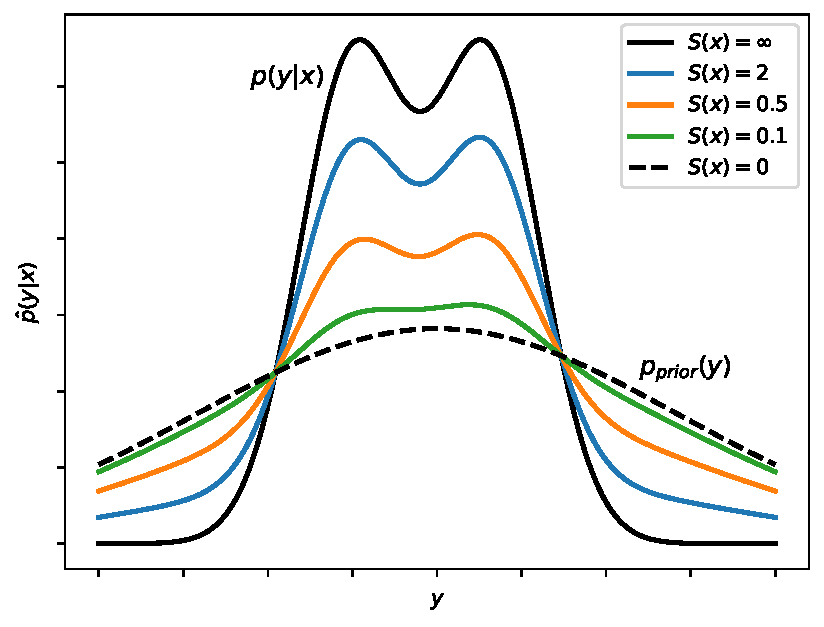
\includegraphics[trim=0.3cm 0cm 0.1cm 0.2cm,clip,width=0.49\textwidth]{Pictures/mixture_predictive_bayesian.pdf}
    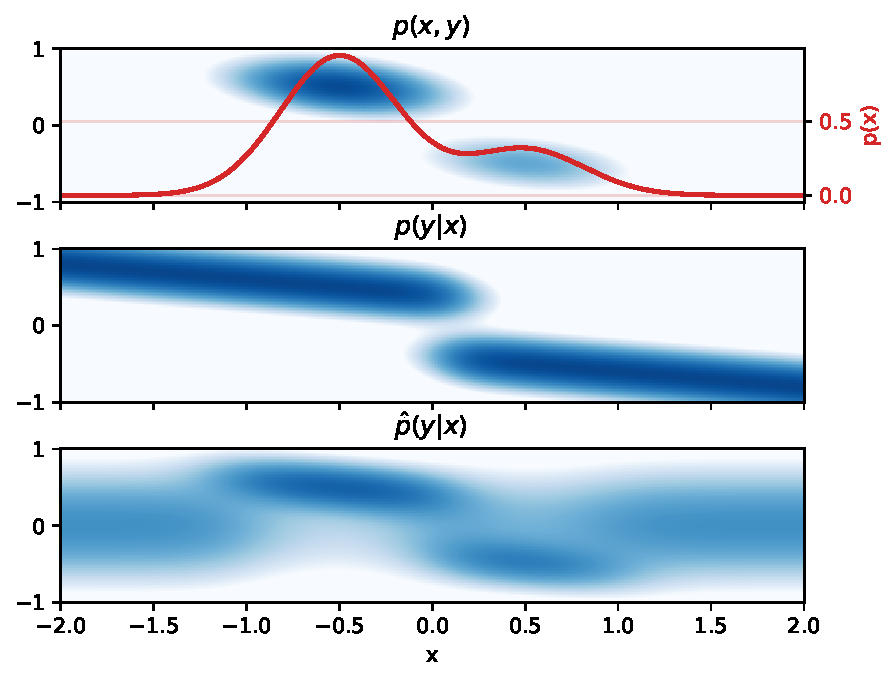
\includegraphics[trim=0.3cm 0cm 0.1cm 0.2cm,clip,width=0.49\textwidth]{Pictures/mixture_predictive_bayesian2D.pdf}
    \caption{Left: Illustration of how the preditive distribution is manipulated according
    the the scaling function $S(x) := p(x)\cdot N\cdot \Delta$. Right: Illustration of why it makes
    sense to manipulate the predictive distribution $p(y|x)$, if there is a small amount of input data
    at a region, then the predictive distribution should transform into the uncertain prior}
    \label{pred_dist_manipulation}
\end{figure}

\subsection{Mean and variance of predictive distribution v1}\label{mean_variance_pred_mixture}
If we just are interested in a Gaussian approximation of the predictive
distribution, this can be easily done assuming we know the mean, variance
and the second moment of the conditional distribution, first the predictive mean
is calculate, 
\begin{align*}
    E_{\hat p(y|x)}[y] &= \int y \cdot \left(\alpha_x \cdot p(y|x) + (1-\alpha_x) p_{prior}(y)\right) dy\\
    &= \alpha_x\cdot E_{p(y|x)}[y] + (1-\alpha_x)\cdot E_{p_{prior}(y)}[y]
\end{align*}

And the predictive variance is calcualted, using the definition of variance, $V_{\hat p(y|x)}[y] =
E_{\hat p(y|x)}[y^2] - E_{\hat p(y|x)}[y]^2$. So we only need to calculate the second moment, 
\begin{align*}
    E_{\hat p(y|x)}[y^2] &= \int y^2 \cdot \alpha_x \cdot p(y|x) + (1-\alpha_x) p_{prior}(y) dy\\
    &=\alpha_x \cdot E_{p(y|x)}[y^2] +(1-\alpha_x) \cdot E_{p_{prior}(y)}[y^2] \\
    &=\alpha_x \cdot(Var_{p(y|x)}[y]+E_{p(y|x)}[y]^2) + (1-\alpha_x) Var_{p_{prior}(y)}[y]
\end{align*}
Assuming $E_{p_{prior}(y)}[y] = 0$. 

\begin{tcolorbox}[
    sharp corners,
    boxrule=0mm,
    enhanced,
    borderline west={4pt}{0pt}{gray},
    colframe=drGray,
    colback=drGray,
    coltitle=black,
]
{\large \textbf{Note: Implementation}}\\
    If we use $\alpha_x \propto p(x)$, then it is not necessary to calculate the conditional
    distribution at all. Assuming $c$ is a constant in $y$. 

    $$\hat p(y|x) = \frac{c\cdot p(x)\cdot  p(y|x) + p_{prior}(y)}{c\cdot p(x)+1} = \frac{c \cdot p(x,y) + p_{prior}(y)}{c\cdot p(x)}$$
\end{tcolorbox}




%  \begin{figure}[H]
%     \centering
%     {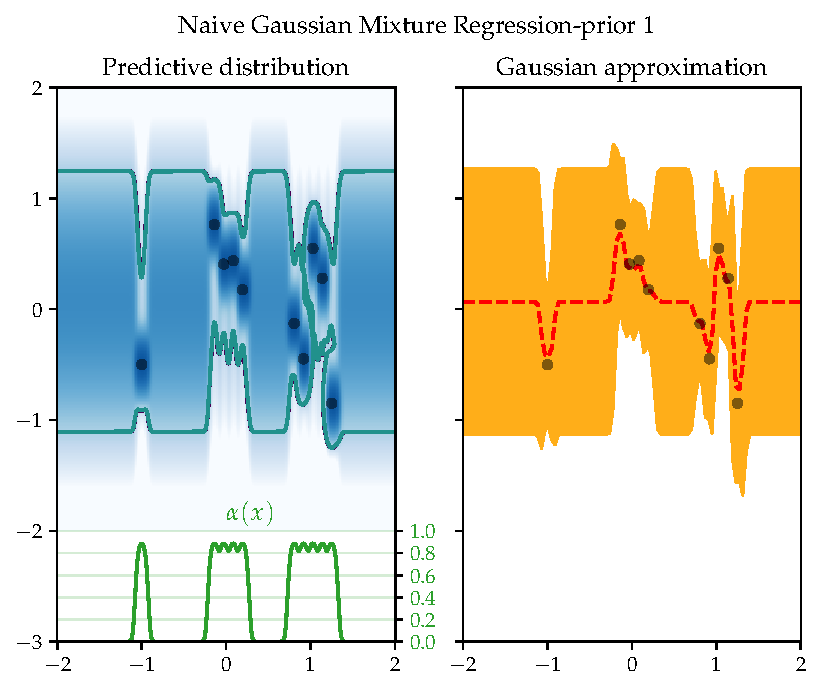
\includegraphics[width=0.46\textwidth]{Pictures/1D_mixture_regression_Naive GMR_N_10.pdf} }%
%     \qquad
%    {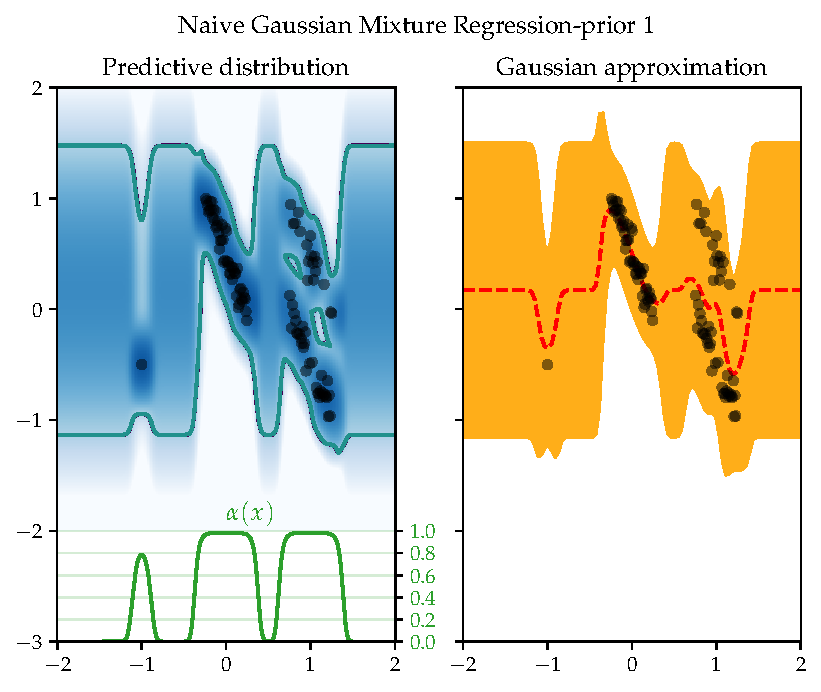
\includegraphics[width=0.46\textwidth]{Pictures/1D_mixture_regression_Naive GMR_N_100.pdf} }%
%     \caption{Example of Naive GMR with prior. When data is observed $\alpha := \frac{S(x)}{S(x)+1}$ gets close
%     to 1 and the likehood is dominant.}
% \end{figure}


\section{Conditional of mixture model}\label{Conditional_mixture}
To exploit a generative model as a surrogate model in Bayesian optimization, we need to calculate
the condtional distribution. Fortunately, all generative models used in this thesis are mixture
models, which simplifies the upcomming deveriations. We define a general mixture model with $Z$ mixture
components as, 
$$p(x,y) = \sum_{z=1}^Z \lambda_z p_z(x,y)$$ where $p_z(x,y)$ are mixture components, i.e. simpler
generative models with same support, $(x,y) \in \mathcal{X}\times \mathbb{R}$. 
The goal is to define
the conditional distribution exact for all the mixture models. As we will soon see, this is again a
mixture model, 
$$p(y|x) = \sum_z \gamma_z(x) p_z(y|x).$$ with $\sum_z \gamma_z(x) = 1$ and $\gamma_z(x) \in [0,1]$.
First, we calcalculate the marginal distribution $p(x)$ of the mixture, 
%assuming that it is possible to marginalize $p_z(x) = \int p_z(x,y) dy$
\begin{align*}
    p(x) &= \int p(x,y) dy =\sum_{z} \lambda_z \int p_z(x,y) dy =\sum_{z} \lambda_z p_z(x).
\end{align*}

Next, we can calculate the conditional in terms of the conditional of the individual mixture
components, 
\begin{align*}
    p(y|x) &= \frac{p(y,x)}{p(x)}\\
    &= \sum_{z} \frac{\lambda_z}{p(x)} p_z(x,y)\\
    &=  \sum_{z}  \frac{\lambda_z p_z(x)}{p(x)}p_z(y|x)\\
    &=  \sum_{z}  \underbrace{ \frac{\lambda_z p_z(x)}{\sum_{z^*} \lambda_{z^*} p_{z^*}(x)}}_{\gamma_z(x)} p_z(y|x).
\end{align*}

So we see that the conditional of a mixture model is again a mixture model. 
We also see that $\sum_z \gamma_z(x) = 1$ and hence we can interpret the above as the following, 
$$p(y|x) = p_z(y|x),  \hspace*{1cm} z \sim Cat(\gamma_1(x), \dots, \gamma_Z(x)).$$ And we name
$p(z|x) = \gamma_z(x) \in [0,1]$ the \textit{responsibility} of mixture component $z$ at a given
location $x \in \mathcal{X}$, (The probability that $y$ to belong to component $z$ at a given
location $x$). For implementation we notice that the denominator in $\gamma_z(x)$ can be reused for
all components. 

\begin{testexample}[Gaussian approximation of mixture conditional]
    As discussed in Section \ref{mean_variance_pred_mixture}, in order to obtain the closed-form
    solution in the expected improvement, we can approximate the  mixture with a gaussian distribution, 
    i.e. calculation of the conditional mean and variance. 

    The mean of the conditional is just
    \begin{align*}
        E_{p(y|x)}[y] &= \sum_{z} \gamma_z(x) \int y \cdot p_z(y|x)dy \\
        &= \sum_{z} \gamma_z(x) E_{ p_z(y|x)}[y].
    \end{align*}

    The variance is found using the variance definition $V[y] = E[y^2] - E[y]^2$, 
    \begin{align*}
        E_{p(y|x)}[y^2] &= \sum_{z} \gamma_z(x) \int  y^2 p_{z}(y|x) dy \\
        &= \sum_{z} \gamma_z(x) (Var_{ p_z(y|x)}[y]+E_{ p_z(y|x)}[y]^2).
    \end{align*}
\end{testexample}



We will now present all the models and show how their conditional distributions are calculated concretely.

\section{Kernel density estimator regression}
Maybe the most simple mixture model one could think about is to put a small variance Gaussian mixture
component around all data points and weight all the components equally. So for $n$ datapoints,
$\{(x_i,y_i)\}_{i=1}^n$, the generative model is given as, 

$$p(x,y) = \frac{1}{N} \sum_{i=1}^n \mathcal{N}\left(\begin{bmatrix}x\\y\end{bmatrix} \middle|
\begin{bmatrix}x_i\\y_i\end{bmatrix}, \sigma^2 I \right) = \frac{1}{N} \sum_{i=1}^n 
\mathcal{N}(x|x_i, \sigma^2 I)\mathcal{N}(y|y_i, \sigma^2),$$
where $\sigma^2$ is refered as the bandwidth, when the literature refers to the above as a kernel estimator. 
Small $\sigma^2$ yields a complex model and large $\sigma^2$ yields a simple model. Therefore chosing $\sigma^2$
just rigth is crucial for a good model. 


\subsection{Conditional of Kernel density estimator}
Since the kernel density estimator is just a Gaussian mixture model, with no correlation between
any of the variables, yeilding i.e. $p_z(y|x) = p_z(y)$, therefor the conditional distribution is
given as, 
\begin{align}
    p(y|x) &= \sum_{z=1}^n \gamma_z(x) \mathcal{N}(y|\mu_{y}^{(z)},\Sigma_{yy}^{(z)} ),\\
    \gamma_z(x) &= \frac{\lambda_z \mathcal{N}(x|\mu_{x}^{(z)},\Sigma_{xx}^{(z)})}{\sum_{z^*}
\lambda_{z^*} \mathcal{N}(x|\mu_{x}^{(z^*)},\Sigma_{xx}^{(z^*)})}.
\end{align}
The computational complexity of calculating the conditional or the predictive distribution is
$O(n)$, since we reused the denominator of $\gamma_z(x)$ for all components $z$. 

\section{Gaussian mixture regression}
Extending the kernel estimator regression with covariance between the variables, only $K \leq N$ components 
and different weighting on each component, we arrive at a Gaussian mixture model. The conditional of GMM 
gives the Gaussian mixture regression model \cite{GMR}. 

We can model our data, as a generative model $p(x,y)$, 
$$p(x,y)= \sum_{z=1}^K \lambda_z \mathcal{N}(x,y|\mu^{(z)},\Sigma^{(z)}), \hspace{1cm}
\mu^{(z)}=\begin{bmatrix} \mu^{(z)}_x \\ \mu^{(z)}_y \end{bmatrix},\hspace{0.1cm} \Sigma^{(z)} =
\begin{bmatrix} \Sigma^{(z)}_{xx} & \Sigma^{(z)}_{xy}\\ \Sigma^{(z)}_{yx}& \Sigma^{(z)}_{yy}
\end{bmatrix},$$ where $\sum_{z=1}^K \lambda_z = 1$. The parameters $\left(\lambda_z,
\mu^{(z)}, \Sigma^{(z)} \right)_{z=1}^K$ need to be trained, which is done using the EM
algorithm. We will now show how the conditional is calculated exactly. 

\subsection{Conditional of Gaussian mixture model}
Since the components are multivariate Gaussian distributions, we use <REF> and can define the
conditional of a multivariate Gaussian as
\begin{align}
    p_z(y|x) &= \mathcal{N}(y|\mu^{(z)}_{y|x},\Sigma^{(z)}_{y|x} )\\
    \mu^{(z)}_{y|x} :&= \mu^{(z)}_y+\Sigma^{(z)}_{yx}(\Sigma^{(z)}_{xx})^{-1}(x-\mu^{(z)}_x)\\
    \Sigma^{(z)}_{y|x} :&= \Sigma^{(z)}_{yy}-\Sigma^{(z)}_{yx}(\Sigma^{(z)}_{xx})^{-1}\Sigma^{(z)}_{xy}.
\end{align}
Now, the conditional is defined straight forward from Section \eqref{Conditional_mixture},
\begin{align}
    p(y|x) &= \sum_{z=1}^K \gamma_z(x) \mathcal{N}(y|\mu_{y|x}^{(z)},\Sigma_{y|x}^{(z)} ) \\
    \gamma_z(x) :&=\frac{\lambda_z \mathcal{N}(x|\mu_{x}^{(z)},\Sigma_{xx}^{(z)})}{\sum_{z^*=1}^K \lambda_{z^*}
\mathcal{N}(x|\mu_{x}^{(z^*)},\Sigma_{xx}^{(z^*)})}
\end{align}
The computational complexity is $O(K\cdot d^3)$ ($d$ is the dimension of $x$), since the matrix inversion
of the covariance matrix $(\Sigma^{(z)}_{xx})^{-1}$ is the dominating cost and it happens
for all the $K$ components. 

\section{Sum product networks}
%<What is SPN>

A sum-product network (SPN) is a mixture model, which allows for exponentially many mixture
components, but with only <linearly many parameters> and, thereby, tractable inference (i.e.
conditionalization and marginalization queries). In short, the SPN consists of a computational
graph, with tractable leaf distributions, which are combined using products and sums nodes,
recursively. To keep the inference of the SPN tractable, we want to maintain certain properties when
designing the SPN graph. First we need to define a scope. 
\begin{testexample}[Scope of nodes in SPN]
    A scope (sc) of a leaf node is the set of random variables among each dimension of $x = \{x_1,
    \dots, x_{\text{dim}(x)} \}$ and $y$ of which the leaf distribution,
    $p_i(\cdot)$, defines a distribution function (in our implementation the leaf scopes are all
    singletons). The scope of a sum og product node, $i$, are defined recursively, $sc(i) = \cup_{j \in
    ch(i)} sc(j)$. 
\end{testexample}

\begin{itemize}[noitemsep]
    \item A sum nodes children must have the same scope (completeness). 
    \item A product nodes children must have distinct scopes (decomposability).
    \item Leaf nodes must have tractable inference.
\end{itemize}


The density of the mixture models is calculated in the following way, 
\begin{algorithm}
    \caption*{Calculation of $p(x,y)$}\label{SPN_1}
    \begin{algorithmic}
    \State \textbf{Input:} Fully trained SPN, with leaf distributions $p_i(\cdot)$ for $i\in \mathcal{L}eaf(S)$ and weights 
    $w_{i,j}$ for $(i,j) \in \{(i,j)|i \in \mathcal{S}um(S), j \in ch(i)\}$ 
    \Function{\text{Eval}}{node i}
    \If{$i \in \mathcal{L}eaf(S)$}
        \State  $\textbf{return: } p_i(x,y)$ \Comment{evaluate leaf distributions at point $(x,y)$}
    \EndIf
    %\For{$i \in I_{o}$}
    \If{$i\in \mathcal{S}um(S)$}
        \State $\textbf{return: } \sum_{j\in ch(i)} w_{i,j} \text{Eval}(j)$
    \EndIf
    \If{$i\in \mathcal{P}rod(S)$}
        \State $\textbf{return: } \prod_{j \in ch(i)} \text{Eval}(j)$
    \EndIf
    \EndFunction
    \State $p(x,y) =  \text{Eval(root node)}$
    \end{algorithmic}
\end{algorithm}

In this thesis, we implement the SPN similar to the RAT-SPN presented in \cite{RAT_SPN}, 
which ensures that we have a Complete and decomposable SPN. The following is the structure of 
the RAT-SPN,
\begin{enumerate}[noitemsep]
    \item Define $C$ leaf distributions per random variable\footnote{Note that we define the random
    variables as the dimensions in the joints distribution, i.e. $\{x_1, ..., x_{\text{Dim}(x)},
    y\}$.} ($C$ is called "channels").
    \item Pair up the elements in the set of random variables in a random way. If uneven set, then
    one element pairs with the empty set.
    \item For each pair: Define $C^2$ product nodes by combining each combination of leaf nodes. 
    \item For each pair: Give the $C^2$ product nodes the same $C$ sum node parents. 
    \item Now, pair up the pairs and repeat step 3 (with sum-nodes instead of leaf nodes) and 4.  
    \item At the final iterations: Give the $C^2$ product nodes 1 sum node parent.
\end{enumerate}
 This is a scalable and easy way to construct the SPN. For high-dimensional problems, we can limit the number
of pairs defined in step 2 and instead, combine more of the randomly defined SPNs in several tracks $T$. This allows the
model to be lucky in the case e.g. dimension $x_3$ and $x_5$ was a powerful combination. Figure \ref{SPN_graph_illu}
illustrates the concept of RAT-SPN for only one track $T=1$ (more tracks would shuffle the pairs).

\begin{figure}[H]
    \centering
    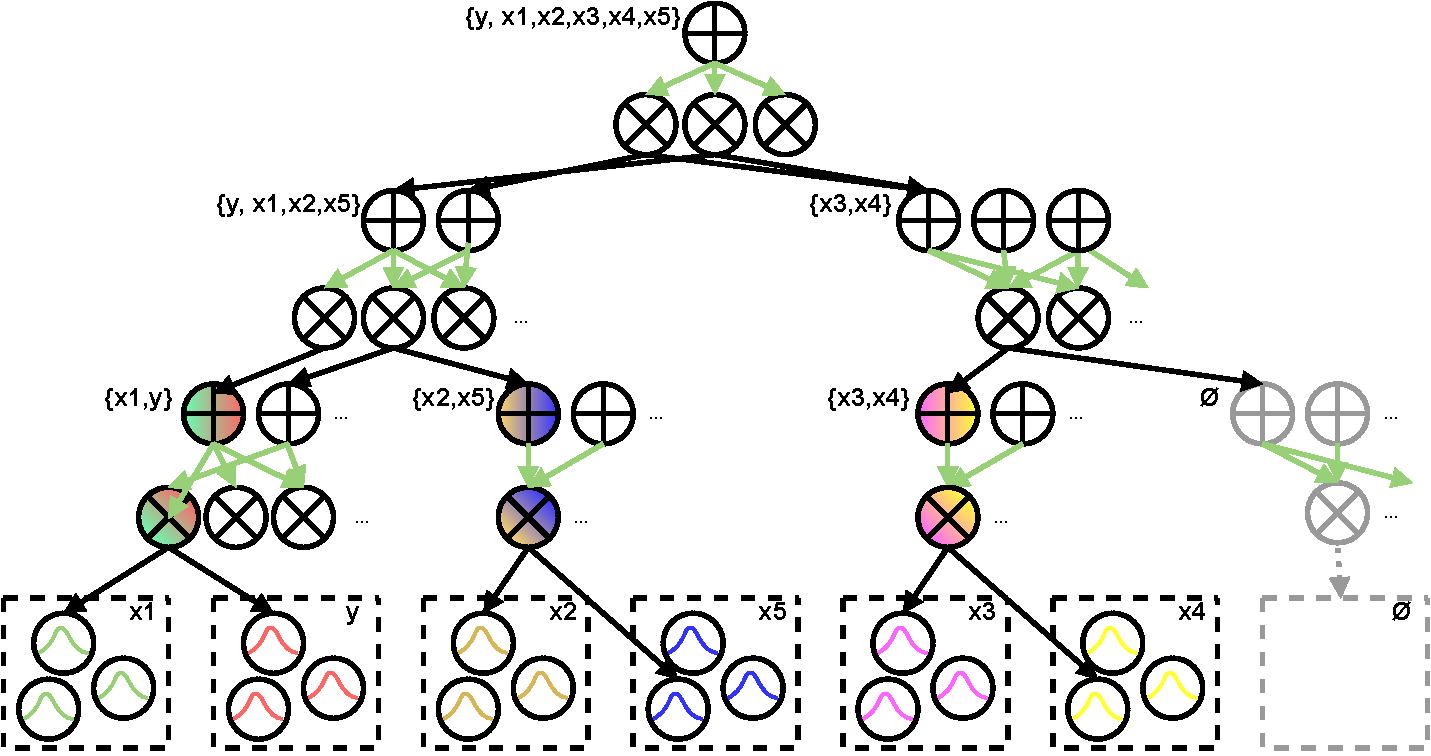
\includegraphics[width=\textwidth]{Pictures/SPN_illustration_graph3.pdf}
    \caption{Illustration of random constructed sum-product network (RAT-SPN) for the joint
    distribution $p(x_1, \dots, x_5, y)$. The product nodes, $\otimes$, always combine 2 nodes from different
    scopes, while sum nodes, $\oplus$, sum all of the product nodes for similar scopes. Note the drawing is not
    complete; This illustarates a RAT-SPN with 3 channels, so every cluster of product nodes has
    size 9 and every cluster of sum nodes (except the root) has size 3.}
     \label{SPN_graph_illu}
\end{figure}

\begin{wrapfigure}{r}{4cm}
    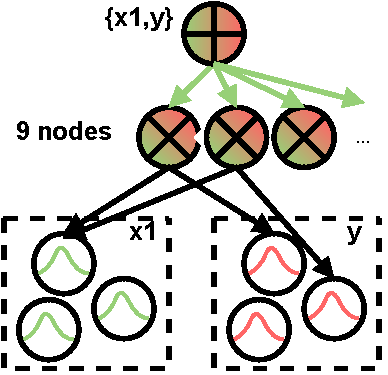
\includegraphics[width=4cm]{Pictures/SPN_illustration_graph1.pdf}
    \caption{Graphical representation of the SPN used in Figure \ref{SPN_fig}. The 9 green arrows
    are weighted and sums to 1}\label{SPN_fig2}
\end{wrapfigure} 
Figure \ref{SPN_fig} illustrates how 3 simple Gaussian distributions from two different scopes $x$ and $y$
can be multiplied together and defined as many mixtures as the product of the numbers of
distributions in each scope (i.e. 9). So by only training parameters for 6 distributions 
we obtain 9 distributions. In the middle figure, we see a data distribution with no need for all 9 
mixture components and the weighting ensures that the unnecessary components are turned off. Figure \ref{SPN_fig2}
illustrates the graphical representation of the SPN for 2 dimensions - and shows that the SPN for small dimensions 
is not deep or complicated. In fact, if we look at the right figure in Figure \ref{SPN_fig}, the SPN is just 
adding less flexibility.

\begin{figure}[H]%
    \centering
    \begin{minipage}[b]{0.32\textwidth}
      \begin{overpic}[trim=0.3cm 0cm 0.1cm 0.7cm,clip,width=\textwidth]{Pictures/SPN_illustration1.pdf}
        \put (-5,40) {\small y}
        \put (40,0) {\small x}
    \end{overpic}
    \end{minipage}
    \hfill
    \begin{minipage}[b]{0.32\textwidth}
      \begin{overpic}[trim=0.3cm 0cm 0.1cm 0.7cm,clip,width=\textwidth]{Pictures/SPN_illustration3.pdf}
        \put (40,0) {\small x}
    \end{overpic}
\end{minipage}
\hfill
\begin{minipage}[b]{0.32\textwidth}
    \begin{overpic}[trim=0.3cm 0cm 0.1cm 0.7cm,clip,width=\textwidth]{Pictures/SPN_illustration2.pdf}
        \put (40,0) {\small x}
    \end{overpic}
      \end{minipage}
    \caption{SPN on the joint probalility $p(x,y)$ with 3 leaf distributions in each scope (shown on
    the axes), trained on 3 different data sets. Left: The data lies perfect for the SPN. Middle:
    Numbers in the graph represent how the weight of each mixture component is weighted. Right: The
    data is distributed badly for the SPN.}%
    \label{SPN_fig}%
\end{figure}


\begin{note2}[SPN as neural network]
     <Lav om> The interpretation of an SPN as a neural network cite{vergari} (what motivated us to look at them in the first place)
    Here, imagine the weights of the sum nodes are parameters, leaf distributions are input neurons, root node is output and
    all other nodes correspond to hidden neurons.
    Note: the depth is at most $\log_2(\# variables)$, yielding not much depth in Bayesian optimization tasks, where the number
    of dimensions typically is small. 
\end{note2}

\subsection{SPN as a mixture model}
Each sum-node can be interpreted as a categorical variable \cite{??}, i.e. a weighted dice. So each
mixture component can be found by starting at the root sum-node and rolling the dice of which green
arrow to continue the path through the SPN. If the path meets a product-node all children are
included in the path. If the path meets a sum-node we roll a dice. Finally, if the path meets a
leaf-node it terminates. The defined path is referred to as a sub-network, $S_z$, in the SPN and is
equivalent to a mixture component. The total number mixture components equal the product of all
sum-nodes children, i.e. $Z = \prod_{i\in \mathcal{S}um(S)}|ch(i)|$. i.e. an exponentially large
amount. 

Denote the set of edges in the sub-network $\mathcal{E}(S_z)$.
Now the we define a mixture coeficient, $\lambda_z$ and component for each $S_z$ as 
$$\lambda_z := \prod_{(i,j)\in \mathcal{E}(S_z)} w_{i,j}, \hspace{1cm} p_z(x,y|\theta) := \prod_{i
\in \mathcal{L}(S_z)} \phi_i(x,y),$$ where $\phi_i(x,y)$ is the leaf distribution at leaf node $i$
paramitised with $\theta$. It can now be proven that the SPN can be interpreted as the following mixture
model, 
$$p(x,y|w,\theta) = \sum_{z=1}^Z \lambda_z(w)p_z(x,y|\theta)$$
i.e. by the weighted sum of all $Z$ sub-networks. 


\subsection{Conditional of SPN}
Conviniently we can define the mixture model as 
\begin{align*}
    p_z(x,y) &= \prod_{i \in x\mathcal{L}eaf(z)} \phi_i(x)\prod_{i \in y\mathcal{L}eaf(z)} \phi_i(y)\\
            &=: p_{z_x}(x) p_{z_y}(y) 
\end{align*}
<obs connect til forgående sections> giving the conditional of the mixture and the responsibility
\begin{align}
    p(y|x) &= \sum_{z=1}^n \gamma_z(x) p_{z_y}(y)\\
    \gamma_z(x) &= \frac{ \lambda_z p_{z_x}(x)}{\sum_{z \in \Sigma(S)} \lambda_z p_{z_x}(x)}
\end{align}
\subsubsection{calculation of responsibility}
The responsibility of a datapoint to belong to one mixture component, is given by
$$\gamma_z(x) = \frac{\lambda_z p_z(x)}{\sum_{z^*} \lambda_{z^*} p_{z^*}(x)}$$
We can prove that the responsibility is equal to the gradient of the log likehood, 
$$L:= \sum_n \log \sum_z \lambda_z \exp \psi_z(x_n)$$
where we define $\psi_z(x_n) = \log p_z(x_n)$. Take the gradient 
$$\frac{\partial L}{\partial \psi_{z}(x_{n})} = \frac{\lambda_z p_z(x_n)}{\sum_{z^*} \lambda_{z^*} p_{z^*}(x)}$$
Note that the gradient easily can be found using automatic differentiation. 


% \begin{figure}
%     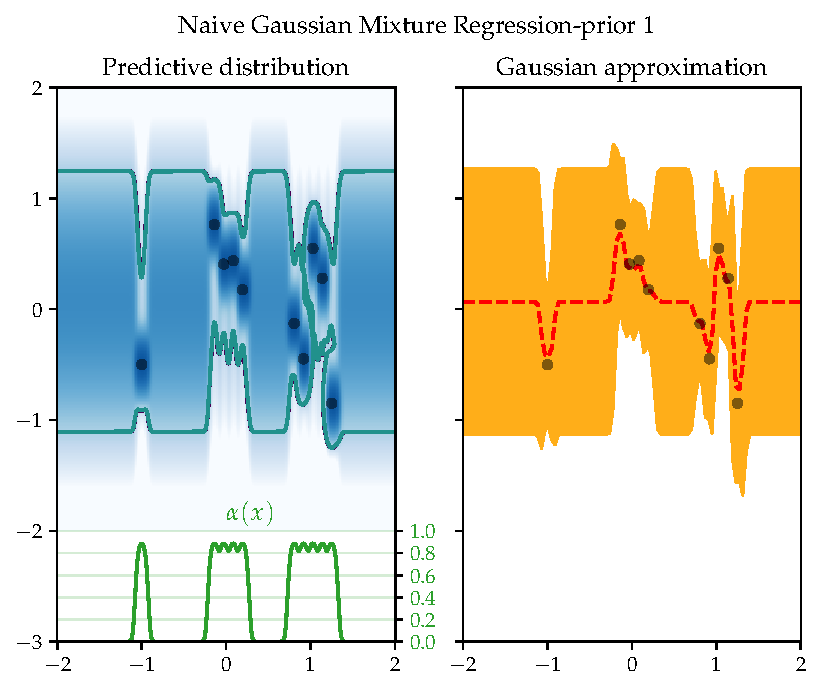
\includegraphics[width=0.5\textwidth]{Pictures/1D_mixture_regression_Naive GMR_N_10.pdf}
% \end{figure}

% \subsection{Conditional of SPN}

% We will soon see how it is possible to write the conditional distribution as the mixture, 
% $$p(y|x) = \sum_{z \in \Sigma(S)} \gamma(x) p_{z_y}(y)$$
% where $ \Sigma(S)$ is the set of all sub-networks in the SPN, $S$ - \todo{IT IS EXPONENTIALLY LARGE}.  
% And where $p_{z_y}(y)$ is defined through $p_z(x,y)$, 
% \begin{align*}
%     p_z(x,y) &= \prod_{l \in \mathcal{L}eaf(z_x)} \phi_l(x)\prod_{l \in \mathcal{L}eaf(z_y)} \phi_l(y)\\
%             &=: p_{z_x}(x) p_{z_y}(y) 
% \end{align*}
% where $\phi_l$ is the density of the $l$'th leafs tractable distribution. Recall that we can interpret an SPN
% as the mixture model, 
% $$p(x,y) = \sum_{z \in \Sigma(S)} \lambda_z p_z(x,y)$$
% where $\lambda_z = \prod_{(q,j) \in \mathcal{E}(z)} w_{q,j}$. First we calculate the marginal density,
% $p(x)$, 
% \begin{align*}
%     p(x) &= \int p(x,y)dy\\
%     &= \int \sum_{z \in \Sigma(S)} \lambda_z p_z(x,y)dy\\
%     %&= \sum_{z \in \Sigma(S)} \lambda_z  \int p_z(x,y)dy\\
%     &= \sum_{z \in \Sigma(S)} \lambda_z p_{z_x}(x)\int p_{z_y}(y)dy \\
%     &= \sum_{z \in \Sigma(S)} \lambda_z p_{z_x}(x)
% \end{align*}
% Now we are ready to calculate the conditional density, 
% \begin{align*}
%     p(y|x) &=  \frac{p(x,y)}{p(x)}\\
%             &= \frac{\sum_{z \in \Sigma(S)} \lambda_z p_z(x,y)}{p(x)}\\
%             &=\sum_{z \in \Sigma(S)}\frac{ \lambda_z p_{z_x}(x)}{p(x)} p_{z_y}(y)\\
%             &=\sum_{z \in \Sigma(S)}\frac{ \lambda_z p_{z_x}(x)}{\sum_{z \in \Sigma(S)} \lambda_z p_{z_x}(x)} p_{z_y}(y)\\
%             &=\sum_{z \in \Sigma(S)} \gamma(x) p_{z_y}(y)
% \end{align*}
% So we defined $\gamma(x) = \frac{ \lambda_z p_{z_x}(x)}{\sum_{z \in \Sigma(S)} \lambda_z p_{z_x}(x)}$ 
% and this is very convinient, as we will see soon is 
% equavalent to the derivative of the log-likehood
% of the SPN, which is easily obtained by automatic differentiation. 


% For convinience
% we define each sum component as $p(z,x,y|w,\theta) := \lambda_z(w)p_z(x,y|\theta)$.
% Evaluation of $p(x,y|w,\theta)$ will never be done as the sum over $Z$ components, 
% instead there is a proposition. 

% \begin{proposition}
%     Consider a SPN, S, a sum node $q \in \mathcal{S}um(S)$ and a child $i \in ch(q)$,
%     then the following relation holds, 
%     $$\sum_{z:(q,i)\in \mathcal{E}(S_z)} \lambda_z(w) p_z(x,y|\theta) = w_{i,q}
%     \frac{\partial S}{\partial v(q)} v(i)$$
% \end{proposition}



% \subsection{SPN as a mixture model}
% <source> we can interpret an SPN as the mixture model, 
% $$p(x,y) = \sum_{z \in \Sigma(S)} \lambda_z p_z(x,y)$$
% where $\lambda_z = \prod_{(q,j) \in \mathcal{E}(z)} w_{q,j}$. And where
% the mixture components are given as 
% \begin{align*}
%     p_z(x,y) &= \prod_{l \in \mathcal{L}eaf(z_x)} \phi_l(x)\prod_{l \in \mathcal{L}eaf(z_y)} \phi_l(y)\\
%             &=: p_{z}(x) p_{z}(y) 
% \end{align*}
% where $\phi_l$ is the density of the $l$'th leafs tractable distribution. The last equation
% is splitting the products up in the two marginals $p_z(x)$ and $p_z(y)$ since they are uncorrelated. 

% The responsibility 
% $$p(z|x) = \frac{ \lambda_z p_{z_x}(x)}{\sum_{z \in \Sigma(S)} }$$
% is calculated easily using autograd. 



%from [@desana]:
% \begin{definition} 
%     A sub-network $\bar S_z$ of $S$ is an SPN, which includes the root $S$ and then includes nodes
%     according to the following recursive scheme: 
% \end{definition}
% \begin{algorithm}[H]
%     \caption*{Collection of sub-network $S_z$ of $S$}\label{SPN4}
%     \begin{algorithmic}
%     %\State \textbf{Global:}  $S_z$ 
%     \Function{Process}{node i, $S_z$}
%     \If{$i \in \mathcal{L}eaf(S)$}
%         \State  $\textbf{return: }$ 
%     \EndIf
%     %\For{$i \in I_{o}$}
%     \If{$i\in \mathcal{S}um(S)$}
%        %\State $S_z =S_z \cup \{j \in ch(i)\}$ \Comment{include one child of node $i$}
%         \State $S_z =S_z.add(j \in ch(i))$ \Comment{include one child of node $i$}
%         \State $\textbf{return: } \text{Process}(j, S_z)$
%     \EndIf
%     \If{$i\in \mathcal{P}rod(S)$}
%         \State $S_z =S_z \cup \{j | j \in ch(i)\}$ \Comment{include all childen of node $i$}
%         \For{$j \in ch(i)$}
%             \State $\textbf{return: } \text{Process}(j,S_z)$
%         \EndFor
%     \EndIf
%     \State $\textbf{return: } S_z$
%     \EndFunction
%     \State $S_z =  \text{Process(root,Ø)}$
%     \end{algorithmic}
% \end{algorithm}






% \section{Gaussian approximation of mixture regression}



% \subsection{Mean and variance of conditional SPN}

% The mean of the conditional is just
% \begin{align*}
%     E_{p(y|x)}[y] &= \sum_{z \in \Sigma(S)} \gamma(x) \int  y p_{z_y}(y) dy \\
%     &= \sum_{z \in \Sigma(S)} \gamma(x) \prod_{l \in \mathcal{L}eaf(z_y)} E_{\phi_l}[y]
% \end{align*}

% and the variance is found using the second moment, 
% \begin{align*}
%     E_{p(y|x)}[y^2] &= \sum_{z \in \Sigma(S)} \gamma(x) \int  y^2 p_{z_y}(y) dy \\
%     &= \sum_{z \in \Sigma(S)} \gamma(x) \prod_{l \in \mathcal{L}eaf(z_y)} (Var_{\phi_l}[y]+E_{\phi_l}[y]^2)
% \end{align*}
\newpage
\section{Mixture model training}
The following section presents the expectation-maximization algorithm, which is used to 
train the Gaussian mixture model and the SPN. 

\subsection{Expectation-maximization for mixture models}
Mixture models can be seen as probibalistic graphical models, <fig> there one mixture component is
picked according to the realization of a catagorical variable $\textbf{Z}$ with parameters according
the the mixture weights, i.e we can reformelate, 
\begin{align}\label{mixture_pdf}
    p(x) &= \sum_{k=1}^K w_k p_k(x)\\
   \iff \hspace*{1cm} p(x) &= p_z(x), \hspace*{0.5cm} z \sim Cat(w_i, \dots, w_K).
\end{align}
In fact $p_z(x)$ is a conditial distribution, $p(x|z)$, and combined with the distribution
of $Z$ we can define the joint 
$$p(x,z):=p_z(x)p(z)$$
The the case of a statistical model, data $\mathcal{D}$ is fitted by the mixture model 
by tuning the model parameters $\theta = \{w, \text{paramers for} p_i\}$. Then the joint
distribtuion $p(\mathcal{D},z| \theta)$ is refered as the \textit{complete-data} likehood in the EM algorithm. 
$$p(\mathcal{D},z|\theta):=p(\mathcal{D}|z,\theta)p(z|\theta)$$ 
When fitting model parameters we essentially want to find the parameters, that maximize the probability of
the parameters given the data, $p(\theta|\mathcal{D})$. Assuming an
unimformative/flat prior $p(\theta)$, 
\begin{align*}
p(\theta|\mathcal{D})&= \frac{p(\mathcal{D}|\theta)p(\theta)}{p(\mathcal{D})}\\
\Rightarrow  \arg\max_{\theta} p(\theta|\mathcal{D}) &= \arg\max_{\theta} p(\mathcal{D}|\theta)
\end{align*}
we arrive at the maximum likelihood estimate (MLE). The task of finding the MLE is conviniently
done using EM algorithm, since we can look at the likehood as the marginalized
\textit{complete-data} likehood, 
$$p(\mathcal{D}|\theta) = \sum_z p(\mathcal{D}, z|\theta)$$

%(Note that this statement true accoring to Theorem 2.1. in \cite{gupta2011theory}). 

\begin{testexample2}[Expectation-maximization EM (based on \cite{bishop})]
    Expectation maximization is a convinient method for finding ML (or MAP) estimate of a 
    latent variable model. We consider a probibalistic model paramitised with $\theta$, 
    $$p(\textbf{X}, \textbf{Z}|\theta)$$ where we denote all latent variables \textbf{Z}, and
    observed variables \textbf{X}. Our goal is to find the maximum of the likehood, 
    $$p(\textbf{X}|\theta) = \int p(\textbf{X}, \textbf{Z}| \theta) \mu(d\textbf{Z})$$
    maximizating the likehood itself $p(\textbf{X}|\theta)$ is assumed dificult 
    but maximizating of the \textit{complete-data} likehood $p(\textbf{X}, \textbf{Z}|\theta)$
    is much easier. The algorithm iterates over two steps: The expecation (E) step and the maximization (M) step, 
    defined in the following way for iteration $t$, 
    
    \textbf{E-step}

    Define the functional $Q(\theta,\theta^{(t)})$, to be the expected value of the complete-data 
    log likehood (log likehood function of $\theta$), with respect to the only random quantaty $\textbf{Z}$,
    which is assumed to follow a distribtuion with the density $p(\textbf{Z}|\textbf{X}, \theta^{(t)})$,
    i.e. the conditional distribution of \textbf{Z} given \textbf{X} and the current parameter point estimate
    $\theta^{(t)}$: 
    $$Q(\theta,\theta^{(t)}) := \mathbb{E}_{p(\textbf{Z}|\textbf{X}, \theta^{(t)})}[\log p(\textbf{X}, \textbf{Z}|\theta)]$$

    \textbf{M-step}

    After the E-step we find the point estimate $\theta^{(t+1)}$ which maximizes $Q(\cdot|\theta^{(t)})$, i.e.
    $$\theta^{(t+1)} = \arg\max_{\theta} Q(\theta|\theta^{(t)})$$

    \begin{algorithm}[H]
        \caption*{(local) maximization of $p(\mathcal{D}|\theta)$}\label{EM}
        \begin{algorithmic}
        \State \textbf{Input:} dataset $\mathcal{D}$, joint model $p(\mathcal{D}, \textbf{Z}|\theta)$
        \While{Not converged}
            \State $Q(\cdot, \theta^{(t)}) \gets \mathbb{E}_{p(\textbf{Z}|\mathcal{D}, \theta^{(t)})}[\log p(\mathcal{D}, \textbf{Z}|\cdot)]$ \Comment{E-step}
            \State $\theta^{(t+1)} \gets \arg\max_{\theta} Q(\theta|\theta^{(t)})$ \Comment{M-step}
        \EndWhile
        \State $\textbf{return: } \theta^{(end)}$
    \end{algorithmic}
    \end{algorithm}

    \textbf{Proof of correctness} 
    
    We will now give a short proof that maximizing $Q(\cdot|\theta^{(t)})$ maximizes the likelihood
    $p(\textbf{X}|\theta)$, where we assume that $\textbf{Z}$ is a random vector with a discrete
    distribution. This allow us to use Gibbs inequality: 
    $$\sum_z p_1(z) \log p_1(z) \geq \sum_z p_1(z) \log p_2(z)$$ where $p_1(\cdot)$ and $p_2(\cdot)$
    are densities belonging to two discrete distributions of $Z$, equality if $p_1(\cdot) =
    p_2(\cdot)$. From now on we will alter the subscript on the expecations, just have in mind that
    $$\mathbb{E}_{\theta^{(t)}}[g(Z)]:=\mathbb{E}_{p(\textbf{Z}|\textbf{X}, \theta^{(t)})}[g(Z)] = \sum_z g(z)
    p(\textbf{z}|\textbf{X}, \theta^{(t)})$$ 
    Now to the proof: From bayes rule $p(\textbf{X}|\theta) =
    \frac{p(\textbf{X}, \textbf{Z})}{p(\textbf{X})}$ we can write
    $$\log p(\textbf{X}|\theta) = \log p(\textbf{X}, \textbf{Z}) - \log p(\textbf{Z}|\textbf{X},\theta)$$
    Now, taking the expecation of the above w.r.t. $p(\textbf{Z}|\textbf{X}, \theta^{(t)})$,
    yields,
    \begin{align*}
        \log p(\textbf{X}|\theta)  &= \mathbb{E}_{\theta^{(t)}}[\log p(\textbf{X}, \textbf{Z}|\theta)]
        -  \mathbb{E}_{\theta^{(t)}}[\log p(\textbf{Z}|\textbf{X},\theta)]\\
        &= Q(\theta,\theta^{(t)})+ \mathbb{E}_{\theta^{(t)}}[\log p(\textbf{Z}|\textbf{X},\theta)]
    \end{align*} 
    Since the above equation holds for any $\theta$, it also holds for $\theta^{(t)}$
    now we have, 
    $$\log p(\textbf{X}|\theta^{(t)}) = Q(\theta^{(t)},\theta^{(t)})+ \mathbb{E}_{\theta^{(t)}}[\log
    p(\textbf{Z}|\textbf{X},\theta^{(t)})]$$ 
    Subtracting the two equations, we get,  
    $$\log p(\textbf{X}|\theta) - \log p(\textbf{X}|\theta^{(t)}) = Q(\theta,\theta^{(t)})
    -Q(\theta^{(t)},\theta^{(t)})+ \mathbb{E}_{\theta^{(t)}}[\log p(\textbf{Z}|\textbf{X},\theta)]-
    \mathbb{E}_{\theta^{(t)}}[\log p(\textbf{Z}|\textbf{X},\theta^{(t)})]$$ 
    From Gibb's inequality we have
    that $\mathbb{E}_{\theta^{(t)}}[\log p(\textbf{Z}|\textbf{X},\theta^{(t)})]\leq \mathbb{E}_{\theta^{(t)}}[\log
    p(\textbf{Z}|\textbf{X},\theta)]$ where equality only holds for $\theta^{(t)} = \theta$, giving
    \begin{align*}
        \log p(\textbf{X}|\theta) - \log p(\textbf{X}|\theta^{(t)}) \geq 
    Q(\theta,\theta^{(t)})
    -Q(\theta^{(t)},\theta^{(t)})
    \end{align*}
    so optimizing $Q(\theta,\theta^{(t)})$ will optimize
    $\log p(\textbf{X}|\theta) $ as least as much.
\end{testexample2}
\newpage
 \subsection{EM for Gaussian mixture}
 For a Gaussian mixture the $p_k$ distributions in \eqref{mixture_pdf} is substituted by Gaussain pdfs, 
 i.e. $p_k(x) = \mathcal{N}(x| \mu_k , \Sigma_k)$
 and the density of a catagorical distribution is $p(z) = \sum_{k=1}^K 1_{z=k} w_k = w_z$, combining the two
 we get the joint distribution, 
 $$p(x,z|w,\mu , \Sigma) = w_z \mathcal{N}(x| \mu_z , \Sigma_z)$$

 Taking the log and defning $\theta = \{\mu_1 , \Sigma_1,w_1, \dots, \mu_K , \Sigma_K, w_K\}$, and assuming iid data
 $$\log p(X,Z| \theta) = \sum_{i}^n \left(\log(w_{z_i})+\log(\mathcal{N}(x_i| \mu_{z_i} , \sigma_{z_i}))\right)$$

Now we are ready to calculate $Q(\theta, \theta^{(t)})$, by taking the expectation of the complete-data log likehood
with respect to the distribution, $p(Z|X, \theta)$, 
\begin{align*}
    \mathbb{E}_{p(Z|X,  \theta^{(t)})}[\log p(X,Z| \theta)] &=\sum_{i}^n  \mathbb{E}_{p(Z|X,  \theta^{(t)})}[p(X_i,Z_i| \theta) ]\\
    &=\sum_{i}^n  \mathbb{E}_{p(z_i|x_i,  \theta^{(t)})}[p(x_i,z_i| \theta) ]
\end{align*}

\begin{note2}[Expectation with repect to unnecessary variables]
    the last equation holds since taking expecation over a function of a random variable $x$ with respect to a that random
    variable and more random variabels, $x,y$, is equivalent to the expecation with respect to just $x$, i.e. 
    \begin{align*}
        \mathbb{E}_{x,y}[g(x)] &= \int\int g(x) p(x,y) dy dx\\
         &= \int g(x) \int p(x,y) dy dx \\
        &= \int g(x) p(x) dy = \mathbb{E}_x[g(x)].
    \end{align*}
\end{note2}
The posterior distribution is calculated the following way,
\begin{align*}
    p(z|x, \theta^{(t)}) &= \frac{p(x,z|\theta^{(t)})}{p(x|\theta^{(t)})} \\
    &= \frac{p(x,z|\theta^{(t)})}{\sum_{z} p(x,z|\theta^{(t)})}\\
    &= \frac{w_z^{(t)} \mathcal{N}(x|\mu_z^{(t)}, \Sigma_z^{(t)})}{\sum_{k=1}^K w_k^{(t)} 
    \mathcal{N}(x|\mu_k^{(t)}, \Sigma_k^{(t)})}
\end{align*}
For simplificaiton we will denote, $\gamma^{(t)}(z_i) := p(z_i|x_i, \theta^{(t)})$, 
interpreted as the probability of datapoint $x_i$ to belong to class $z_i$. Bishop \cite*{bishop}
calls this probability function the \textit{responsibility}. We can now conclude the \textbf{E-step}.

\begin{align*}
    Q(\cdot, \theta^{(t)}) &= \sum_{i=1}^n p(x_i,z_i|\cdot) \gamma^{(t)}(z_i) \\
    &= \sum_{i=1}^n \left[ \gamma^{(t)}(z_i) \log(\cdot_{z_i})+\gamma^{(t)}(z_i) 
    \log(\mathcal{N}(x_i| \cdot_{z_i} , \cdot_{z_i}))\right]
\end{align*}
or more concretely $\theta = \{\mu_1 , \Sigma_1,w_1, \dots, \mu_K , \Sigma_K, w_K\}$, 
$$ Q(\theta, \theta^{(t)}) = \sum_{i=1}^n \gamma^{(t)}(z_i) \log(w_{z_i})+\gamma^{(t)}(z_i) \log(\mathcal{N}(x_i| \mu_{z_i} , \Sigma_{z_i})).$$
$Q(\cdot, \theta^{(t)})$ is a concave function - the Gaussian is log-concave and a sum of concave functions is 
also concave - so it is sufficient and nessesary to find its maxima by the root of its derivative, 
$$\frac{d}{d \theta} Q(\theta^*, \theta^{(t)}) = 0 \iff \theta^* = \arg\max_{\theta} Q(\theta, \theta^{(t)})$$

Giving the updates...

\subsection*{EM for SPN}


% and a normal evaluation of $p(x,y|w_{old}, \theta_{old})$ combined in Bayes rule we obtain
% $$p(z|x,y,w_{old},\theta_{old}) = \frac{p(z,x,y|w_{old},\theta_{old})}{p(x,y|w_{old},
% \theta_{old})} = \frac{\lambda_z(w_{old})p_z(x,y|\theta_{old})}{p(x,y|w_{old}, \theta_{old})} $$

% and we have the expecation for the EM-algorithm, 
% $$Q(\pi, \pi_{old}) = \sum_{n=1}^N \sum_{z=1}^Z p(z|xy_n, \pi_{old}) \ln p(z,xy_n|\pi)$$

\section{Summary}
In the chapter, we introduced the seemingly, novel idea of using a generative model as a surrogate
model in Bayesian optimization. We limited our scope to (Gaussian) mixture models, and quickly
realized the problem of naively using the conditional as a predictive distribution for low-density
areas. This was solved by introducing a prior (background) zero-mean Gaussian with high variance.
How much the prior will influence the predictive distribution will be treated as a hyper parameter
in the upcoming experiements. We continued by deriving the mean and variance of the predictive
distribution (which will be used in the Expected improvement). We shortly introduced the different
mixtures. illustrations of the models (in 1D) are found in the result chapter. The newly rising
class of mixture models, SPNs, were introduced, illustrated and plotted. Finally we also shortly
covered the training of the mixture models, i.e. using the EM algorthm to maximize the likelihood.
With this chapter, we are soon ready to test all the surrogate models, but first,
we need to specify the models more.  